\documentclass[12pt, a4paper]{article}

\usepackage[english]{babel}
\usepackage[utf8]{inputenc}
\usepackage[T1]{fontenc}
\usepackage[table]{xcolor}
\usepackage{booktabs}
\usepackage{url}
\usepackage[colorinlistoftodos,prependcaption,textsize=footnotesize]{todonotes}
\usepackage[a4paper,top=1cm,bottom=1.5cm,left=1cm,right=1cm]{geometry}

\graphicspath{{../img/}}

\setcounter{secnumdepth}{2}
\setcounter{tocdepth}{2}
\makeindex

\begin{document}

\section{Autotuning CACTI Parameters Targeting Area}

We used our Julia autotuning package~\footnote{StochasticSearch.jl:
\url{https://github.com/phrb/StochasticSearch.jl} [Accessed in 10/05/2017]} to
implement an autotuner for the parameters of the CACTI memory modelling tool.
This report summarizes our results.

CACTI models memory access time, cycle time, area, leakage, and dynamic power.
In this initial study we autotuned CACTI parameters for area.  We performed 8
tuning runs of 15 minutes for each of the 3 possible ``cache types'' targeted
by CACTI: ``\texttt{ram}'', ``\texttt{cache}'' and ``\texttt{main-memory}''.

We also present the final values for minimum and maximum power consumption and
access time after we tuned for area. The autotuner aimed to decrease area, but
tuned solutions were also able to decrease power consumption, but not access
time.

\subsection{Relative Area Decrease and Best Value over Time}

\begin{figure}[htpb]
    \centering
    \begin{minipage}{.48\textwidth}
        \centering
        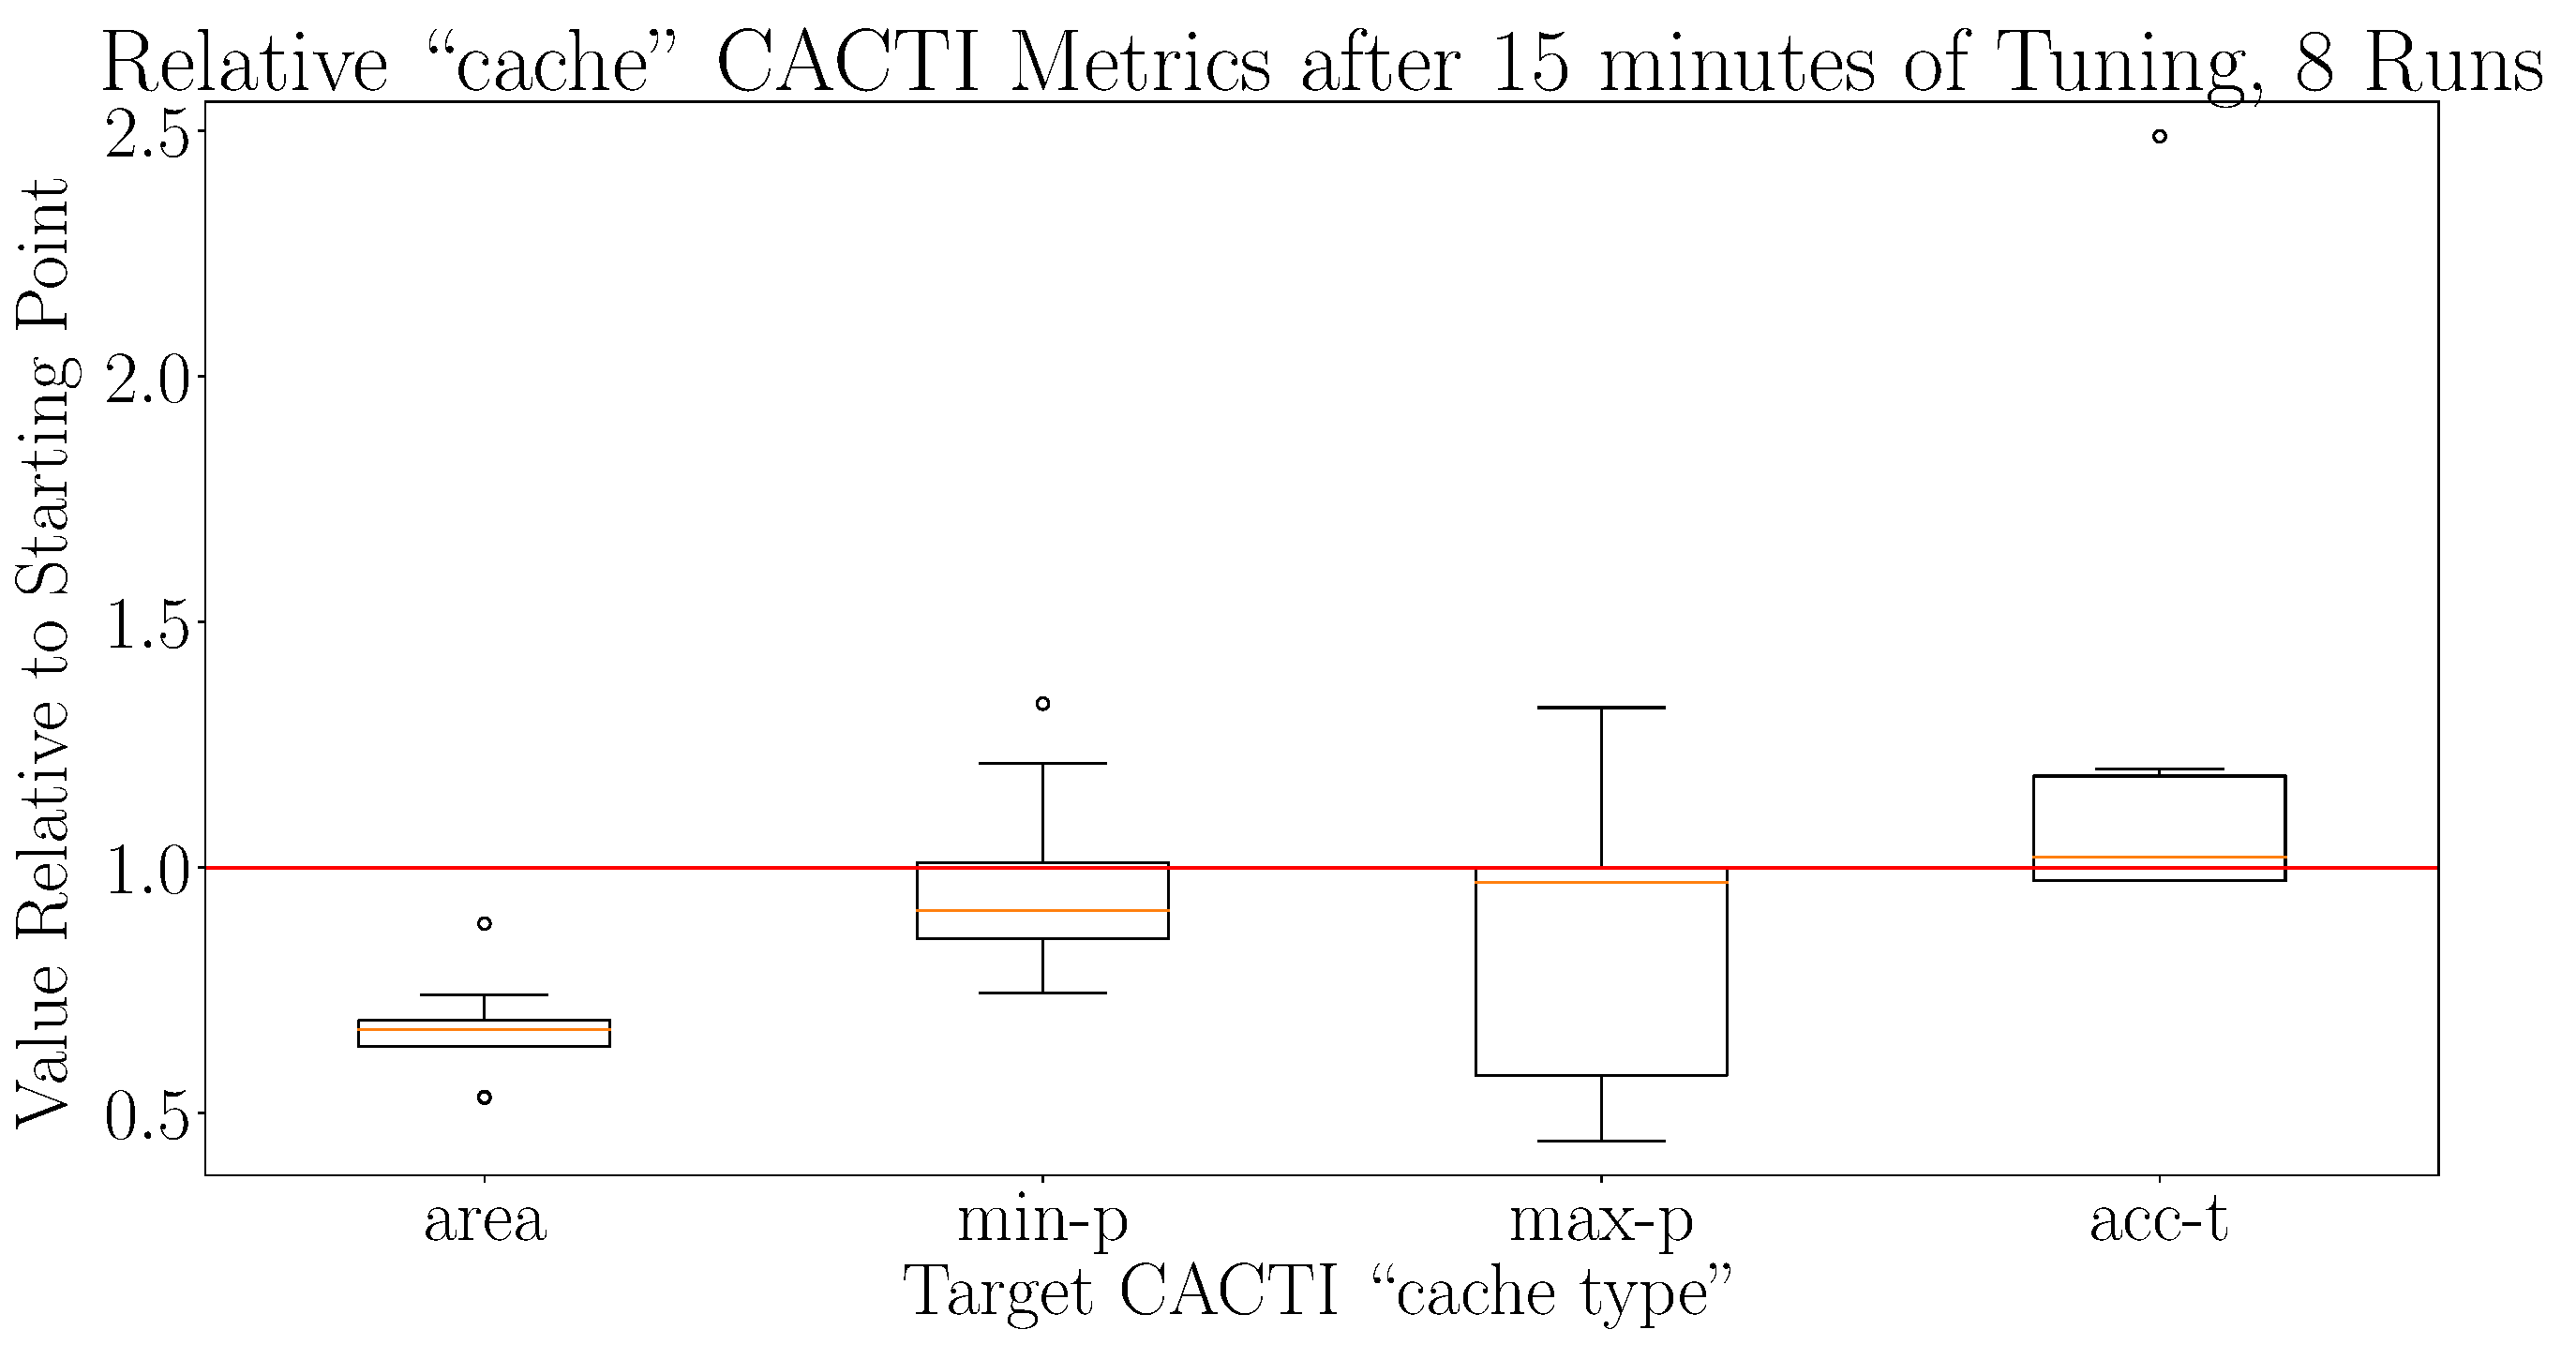
\includegraphics[width=.8\textwidth]{target_area_900_cache}
    \end{minipage}%
    \begin{minipage}{.48\textwidth}
        \centering
        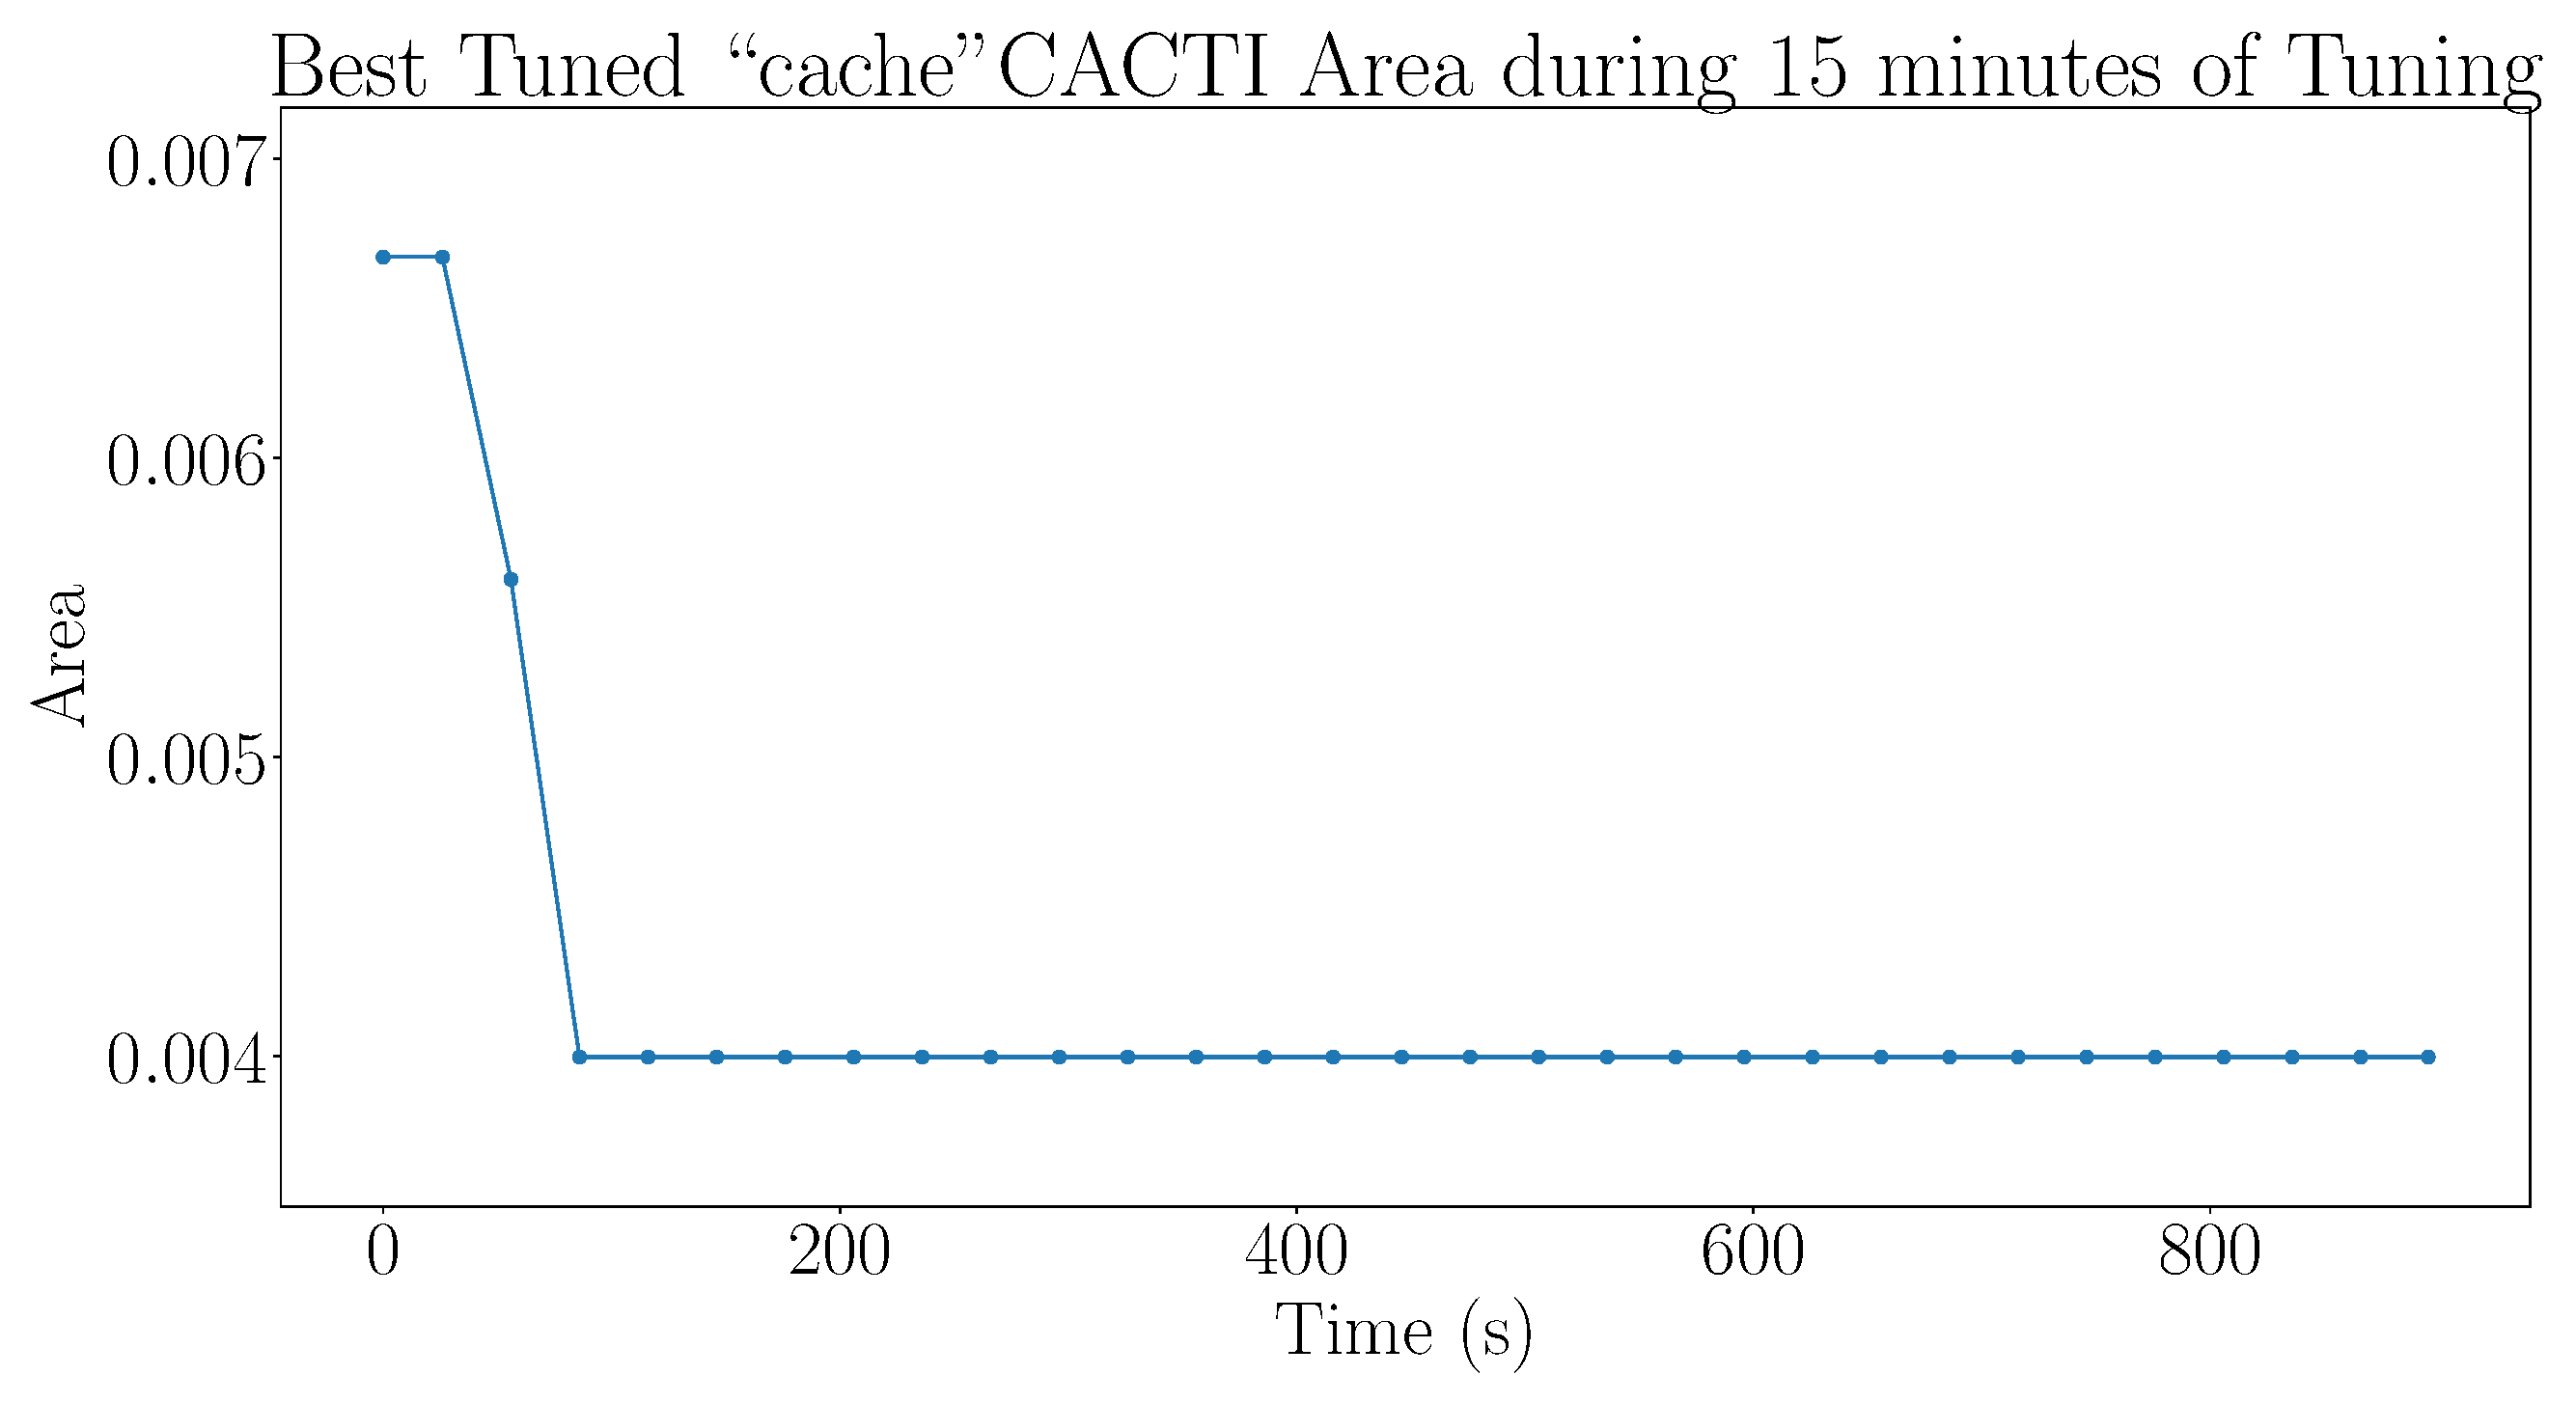
\includegraphics[width=.8\textwidth]{target_area_900_cache_best}
    \end{minipage}%

    \begin{minipage}{.48\textwidth}
        \centering
        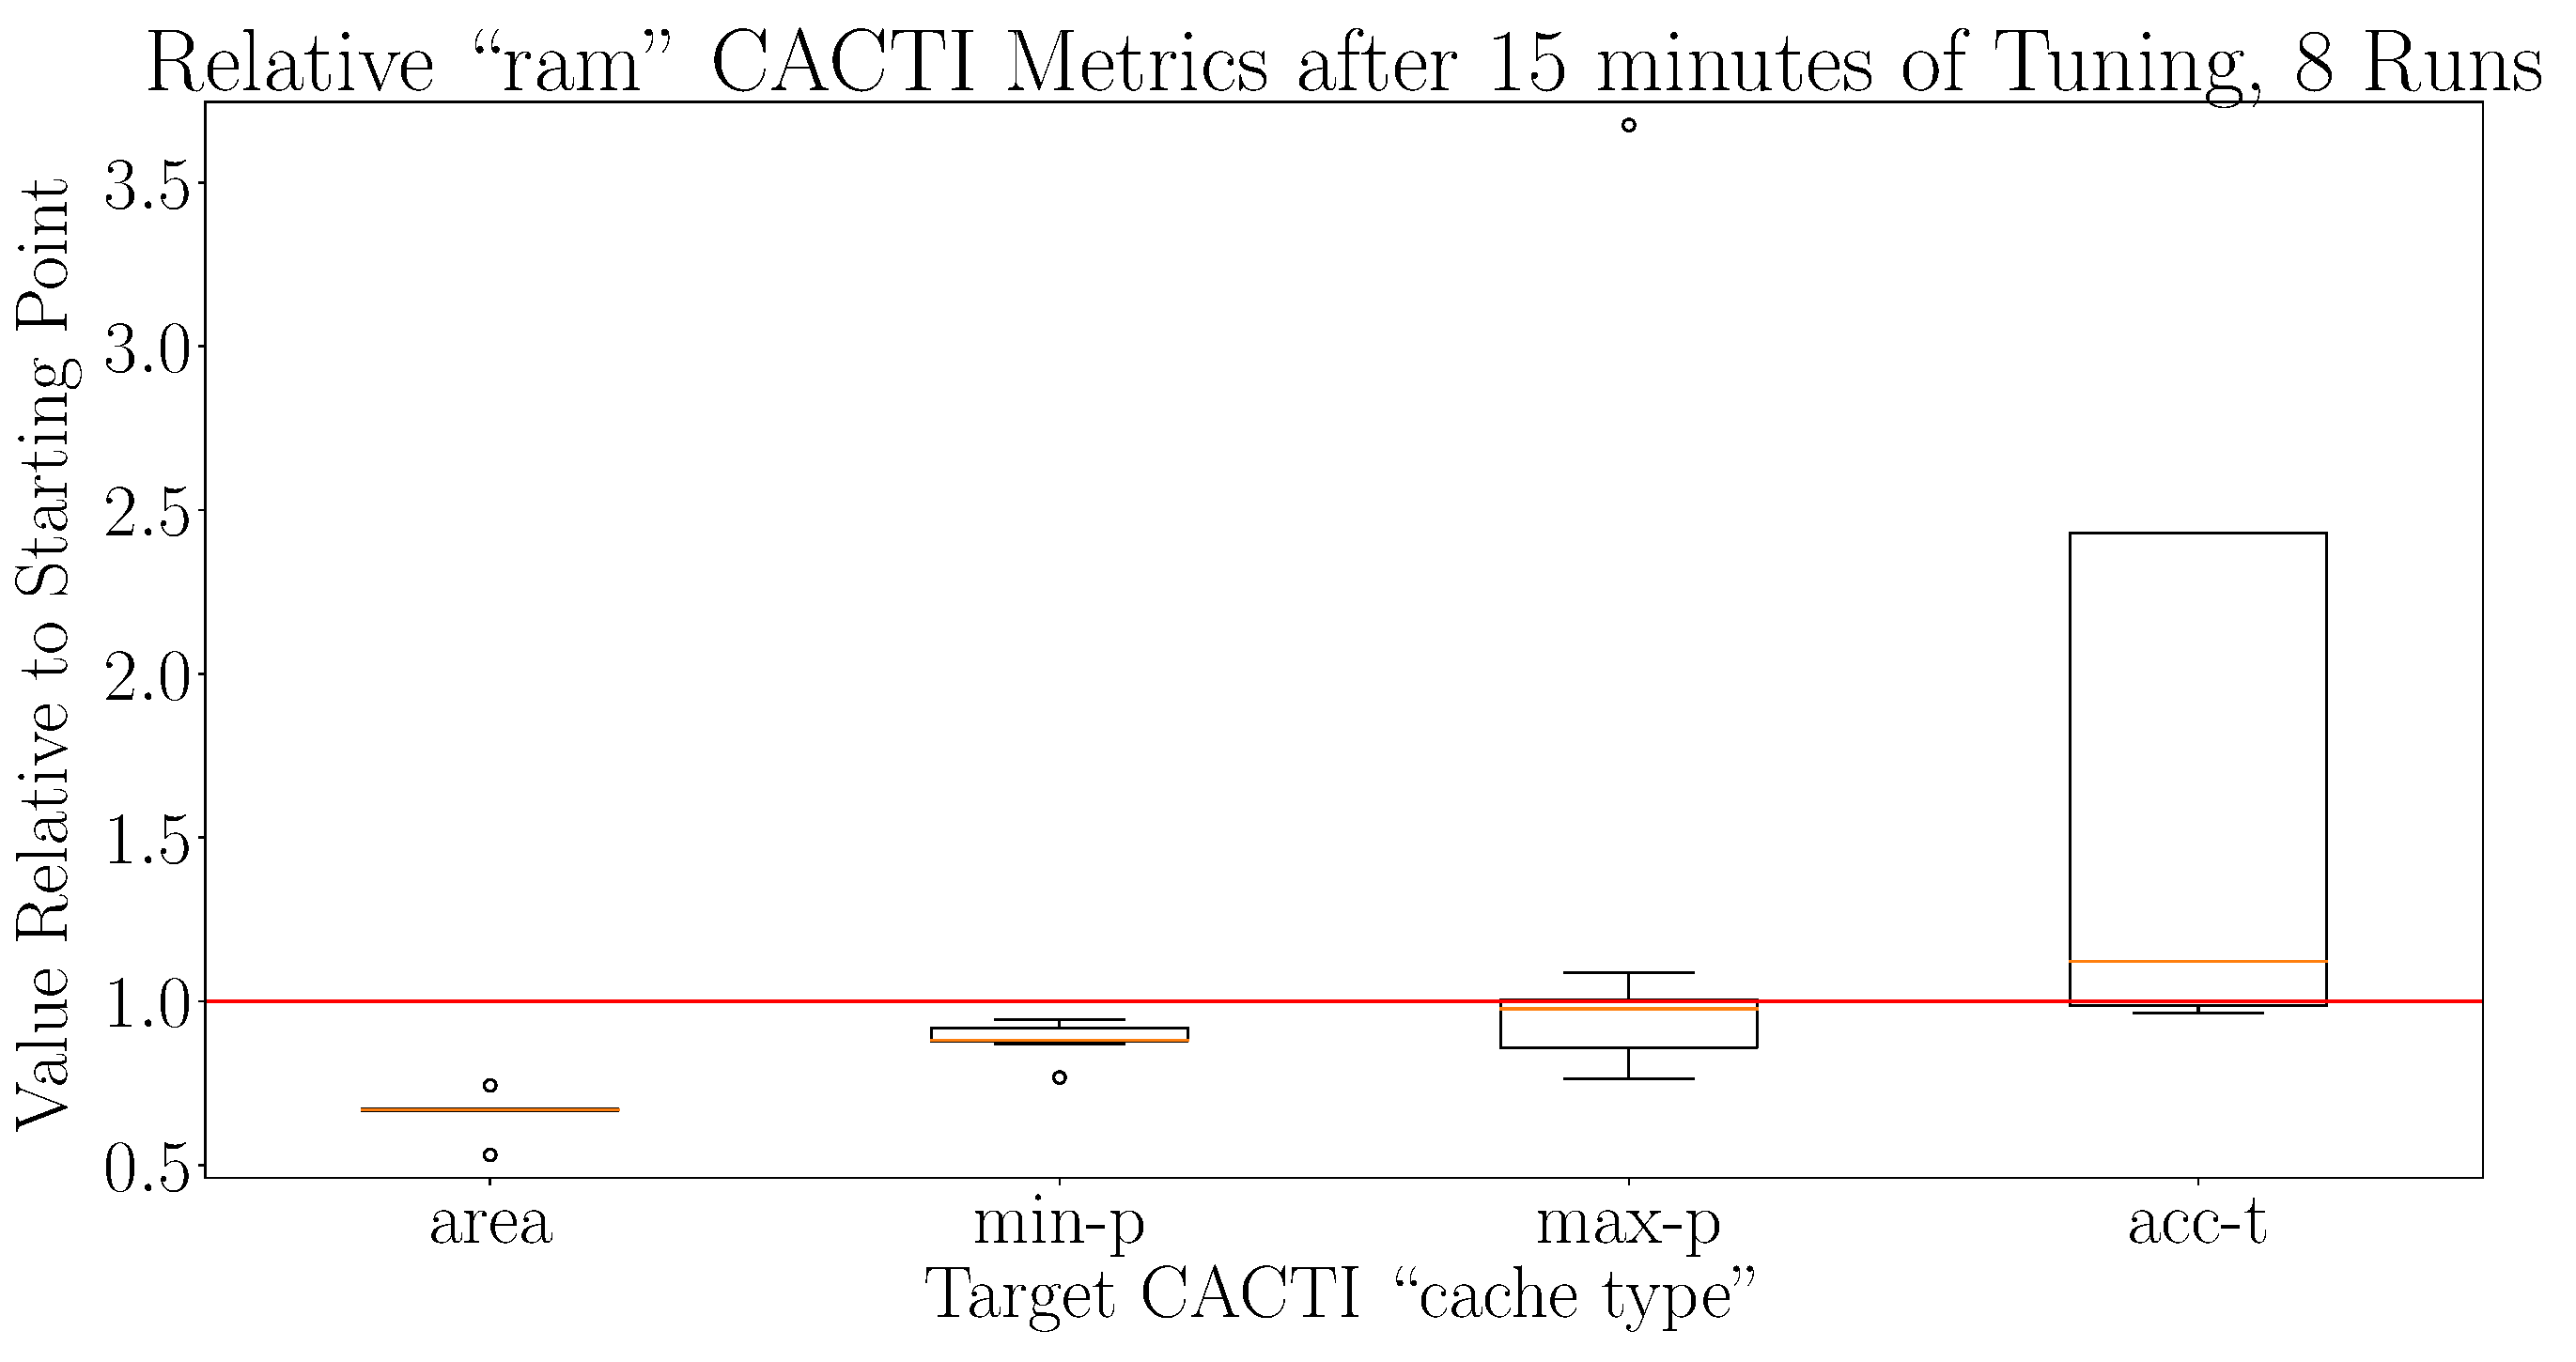
\includegraphics[width=.8\textwidth]{target_area_900_ram}
    \end{minipage}%
    \begin{minipage}{.48\textwidth}
        \centering
        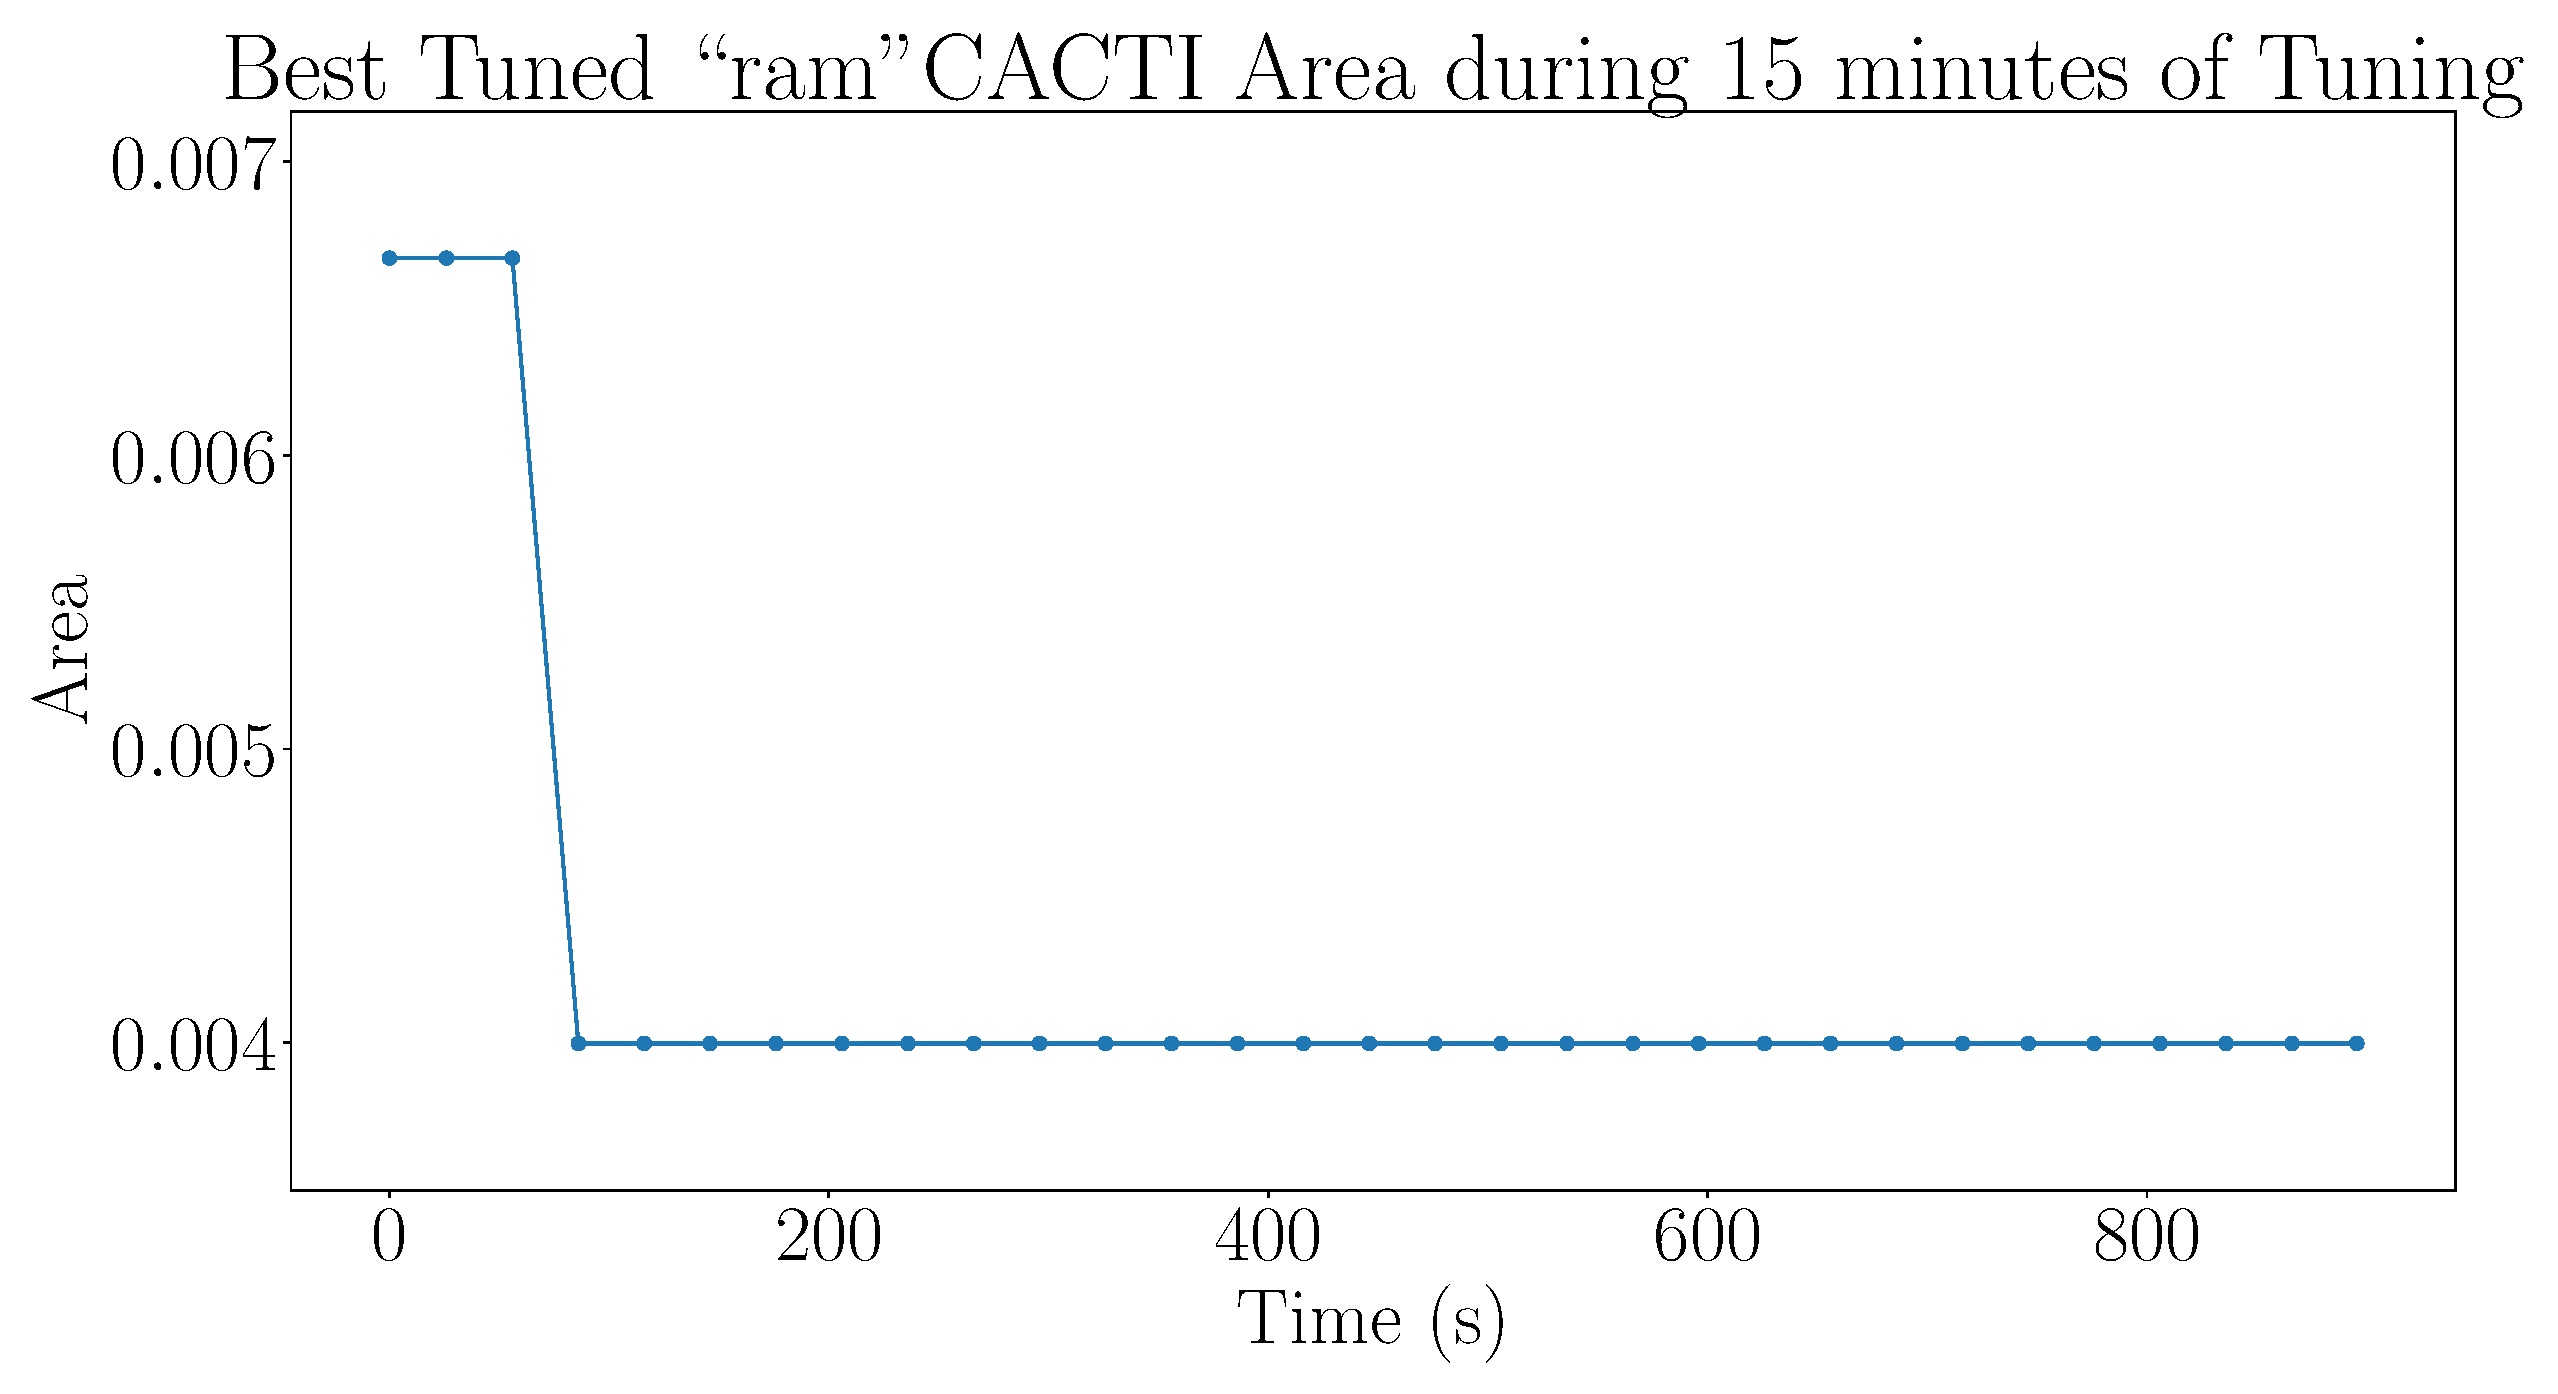
\includegraphics[width=.8\textwidth]{target_area_900_ram_best}
    \end{minipage}%

    \begin{minipage}{.48\textwidth}
        \centering
        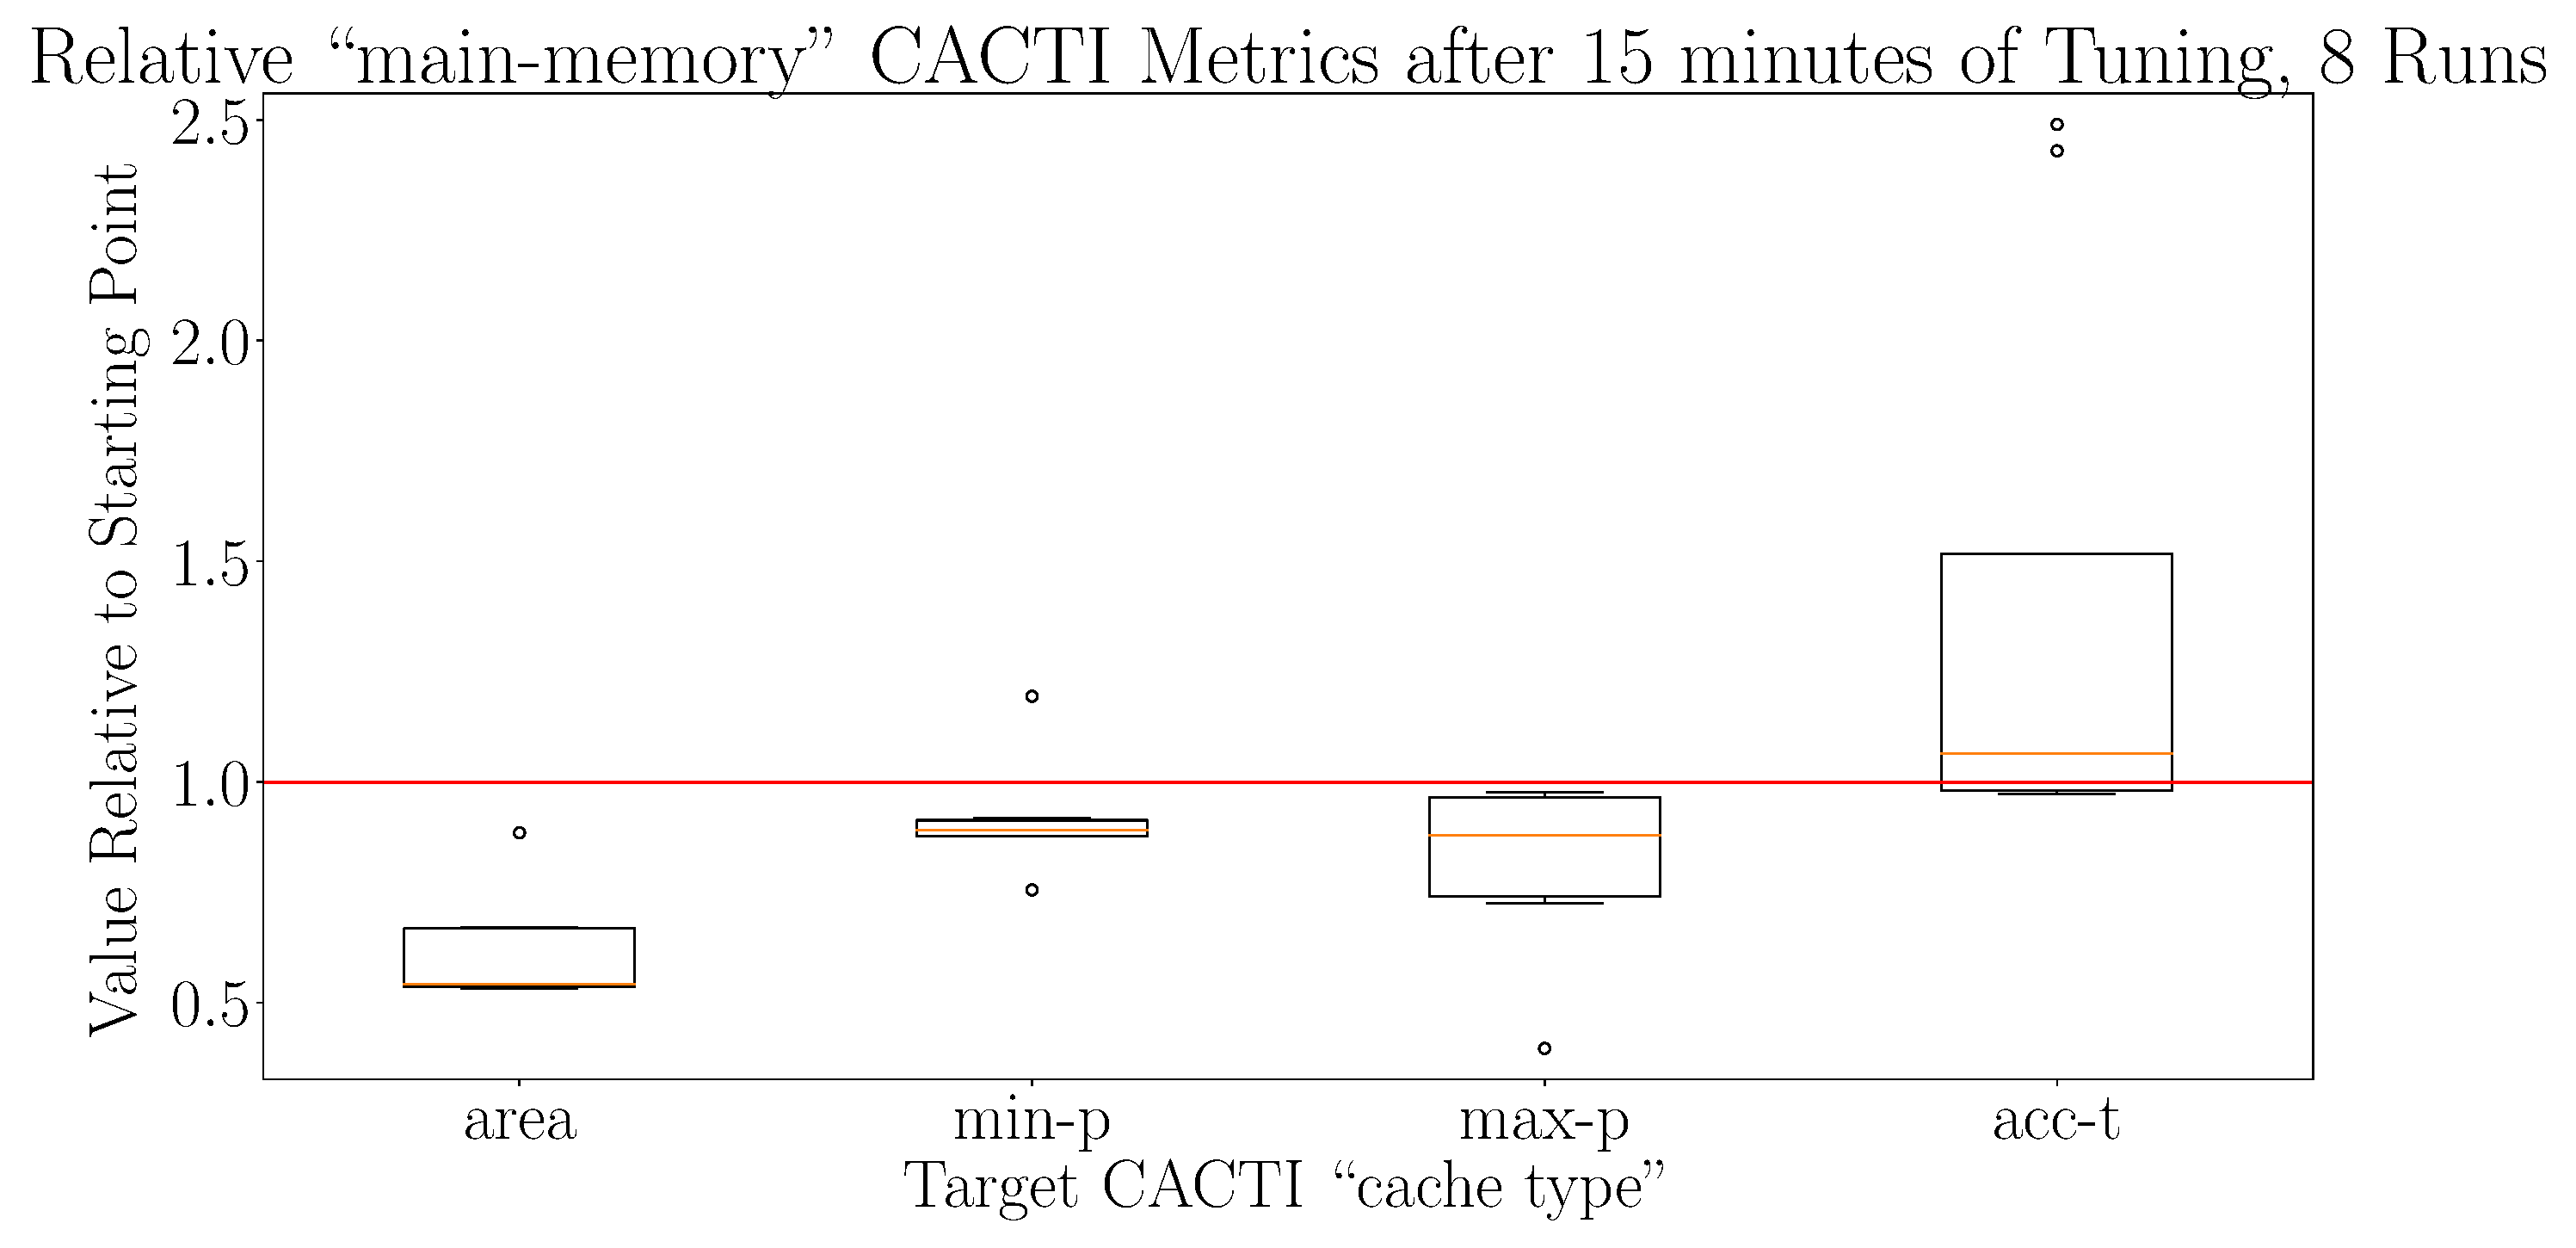
\includegraphics[width=.8\textwidth]{target_area_900_main-memory}
    \end{minipage}%
    \begin{minipage}{.48\textwidth}
        \centering
        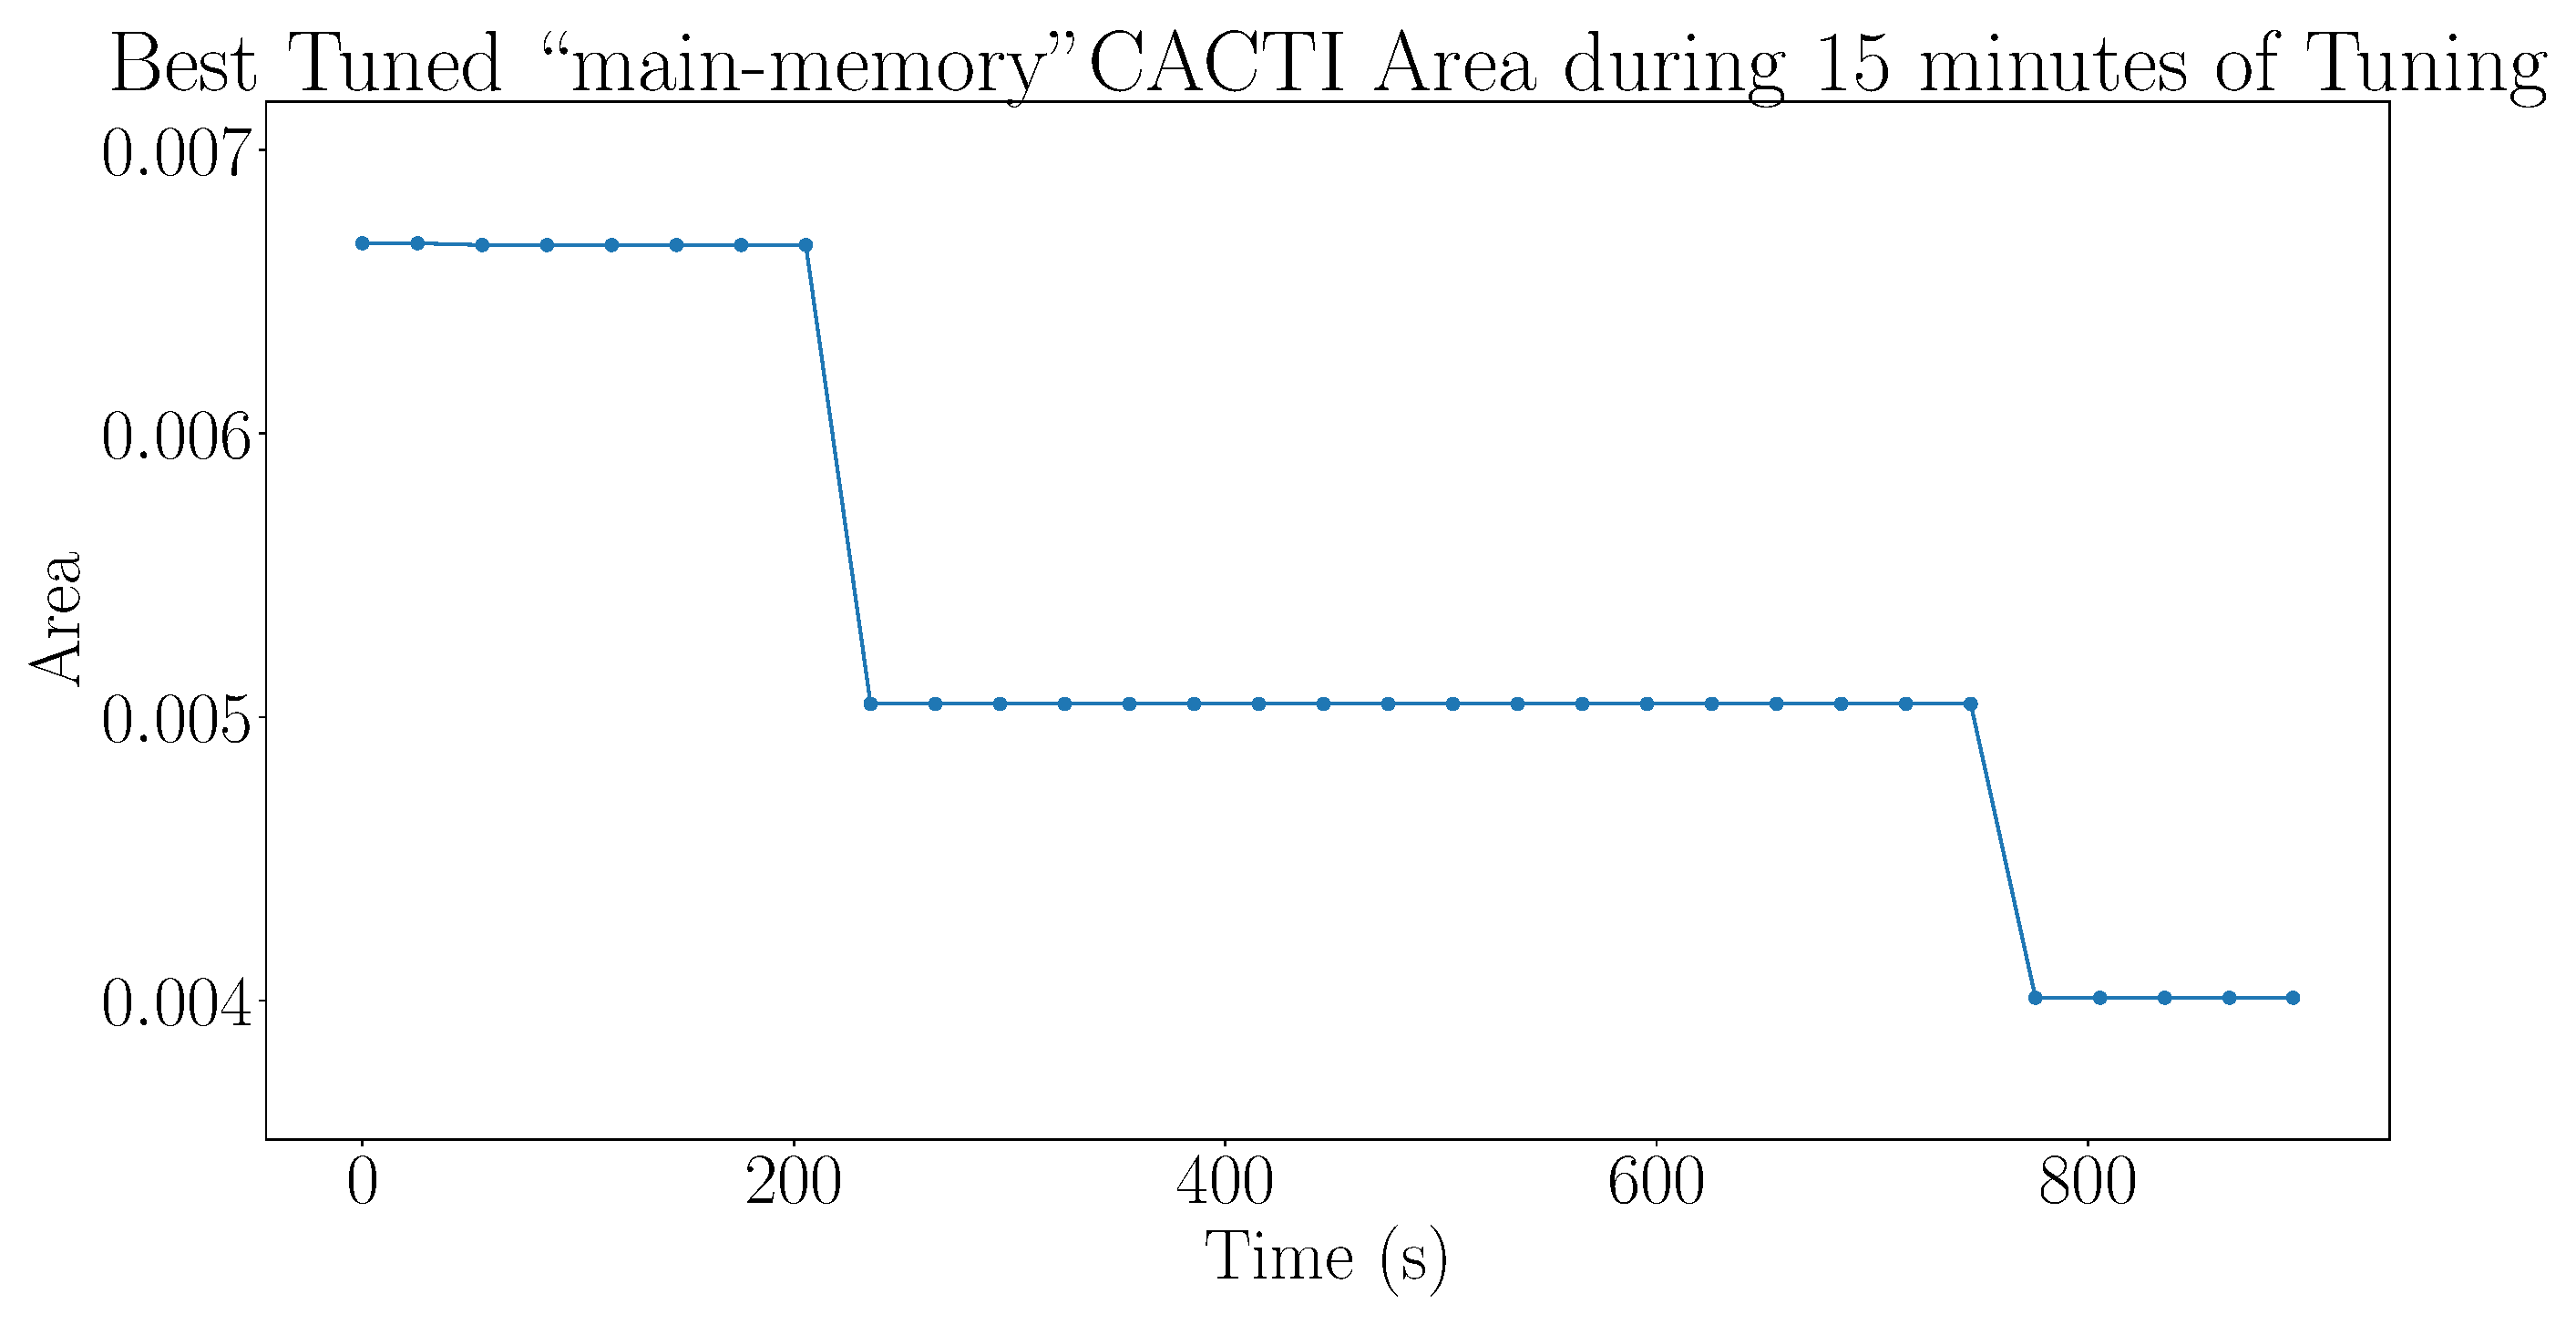
\includegraphics[width=.8\textwidth]{target_area_900_main-memory_best}
    \end{minipage}%
\end{figure}

\begin{figure}[htpb]
    \centering
    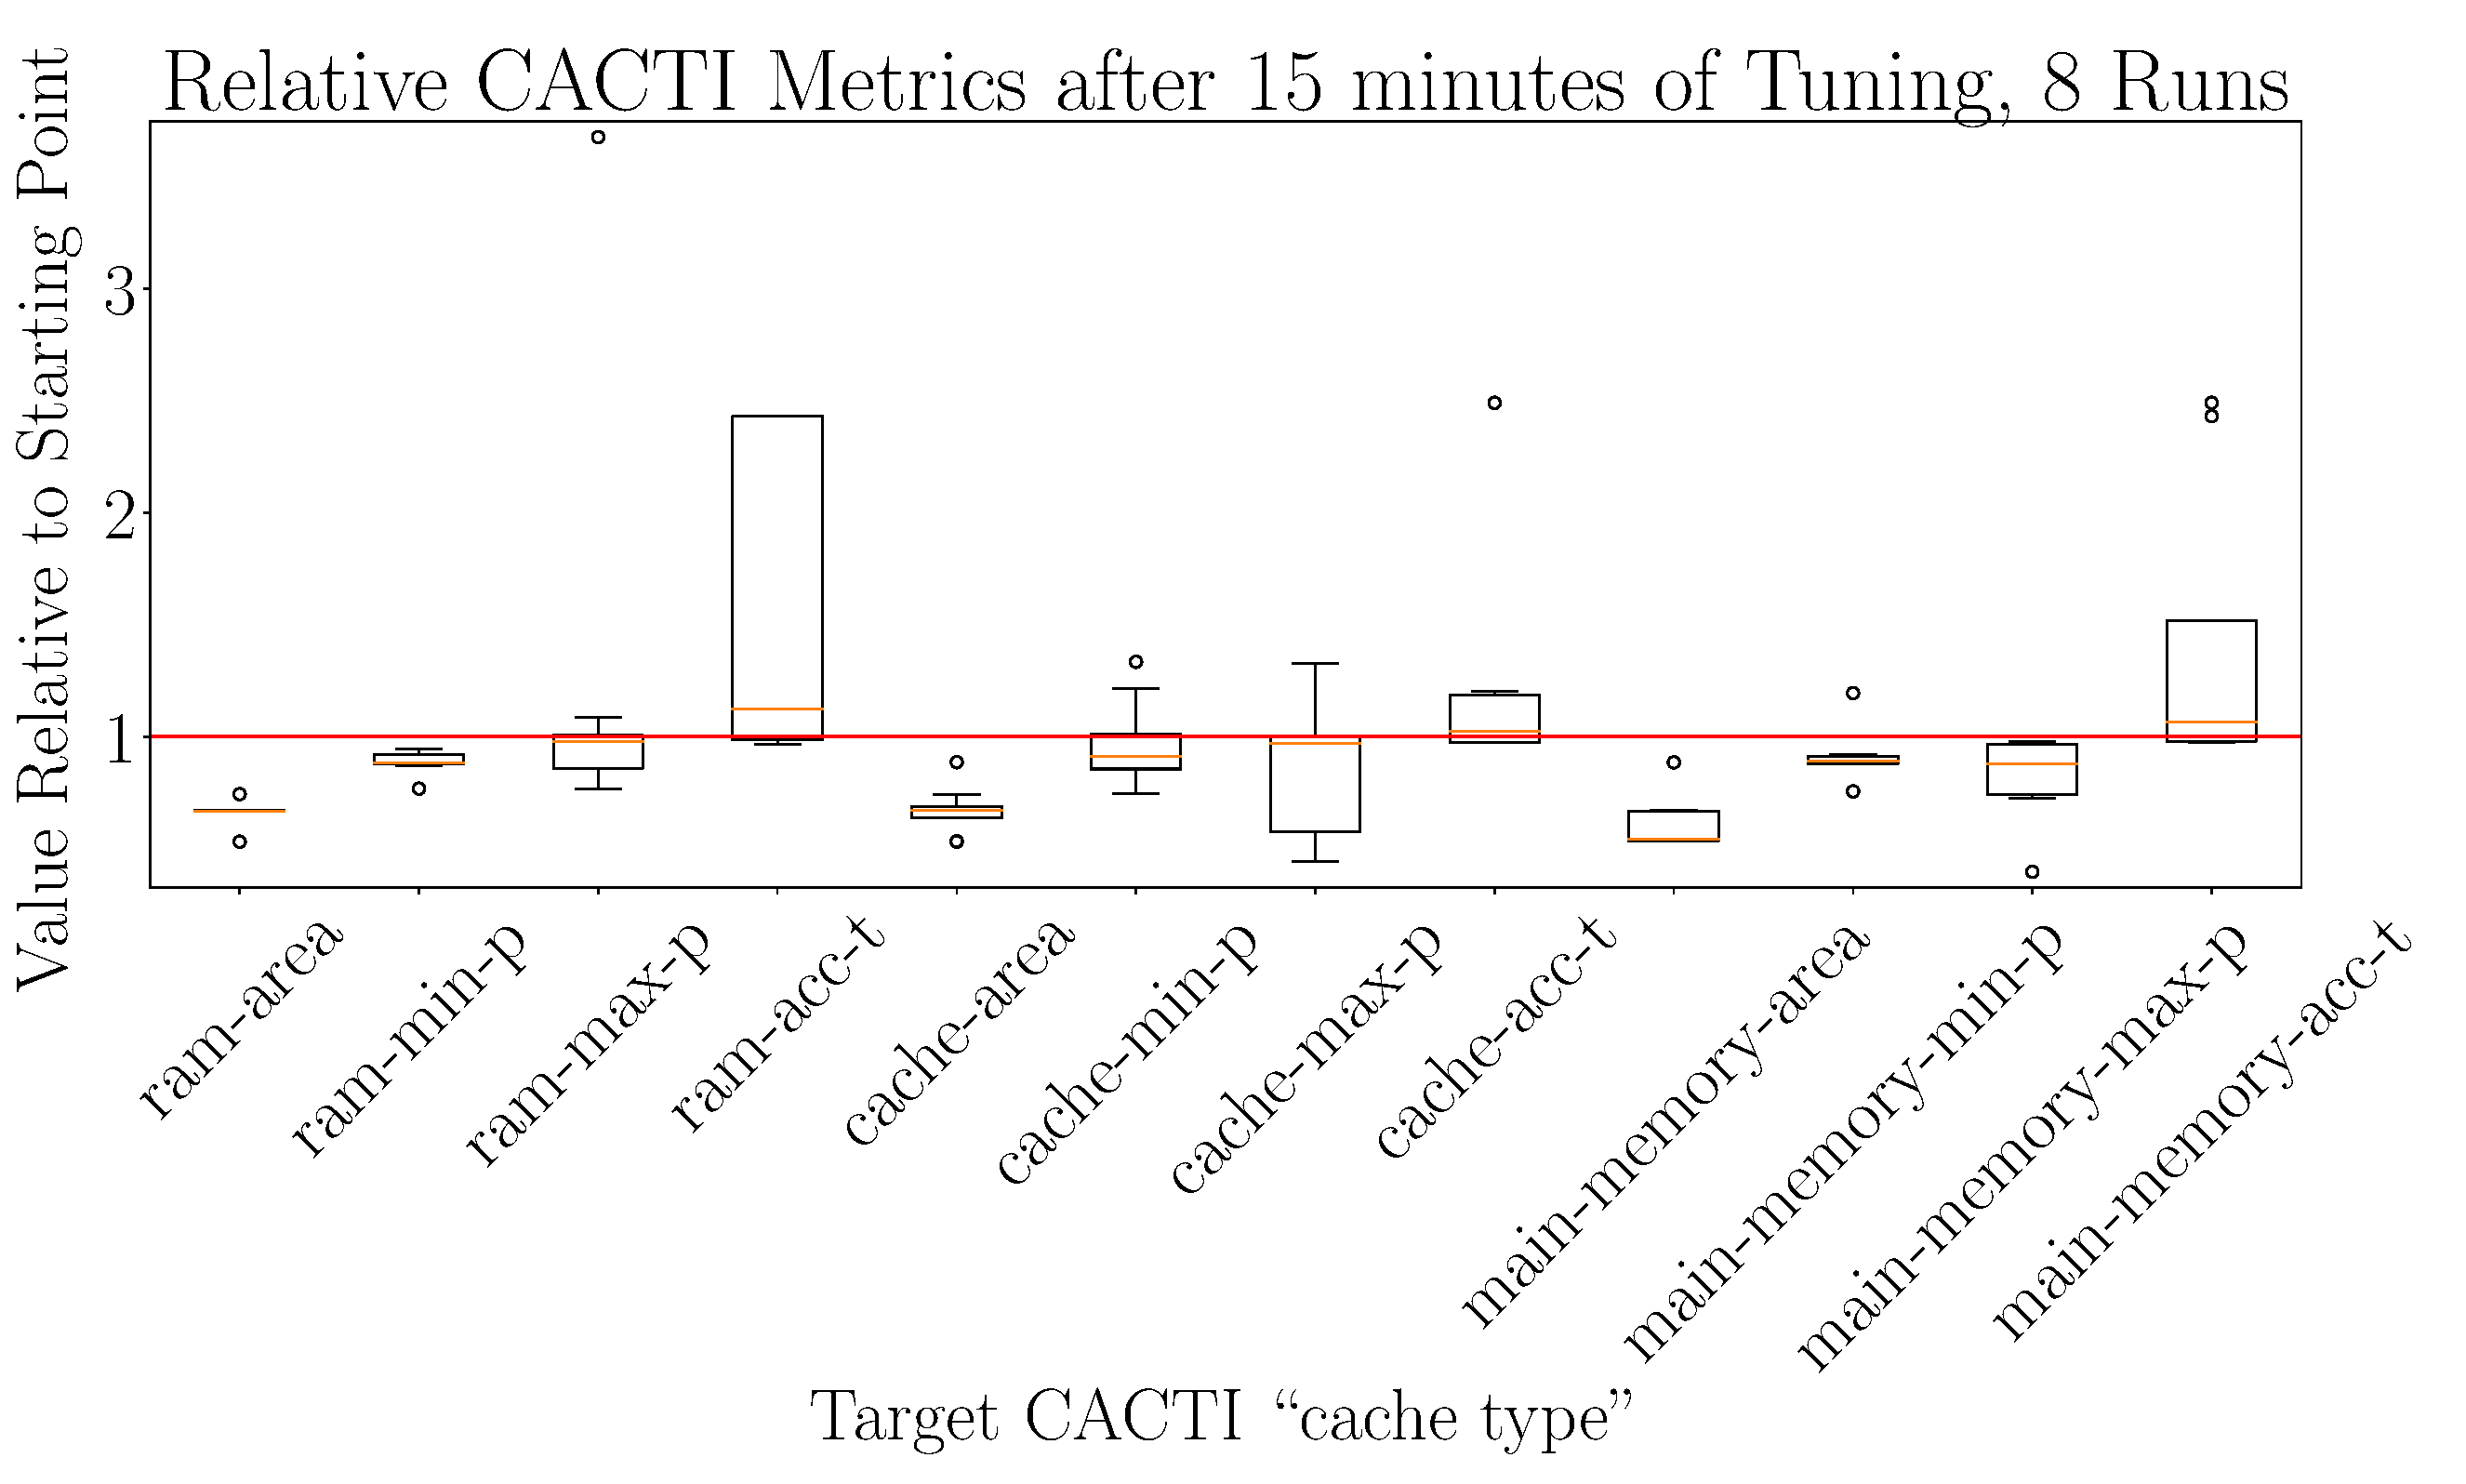
\includegraphics[width=.4\textwidth]{target_area_900}
\end{figure}

\end{document}
